%%%%%%%%%%%%%%%%%%%%%%%%%%%%%%%%%%%%%%%%%%%%%%%%%%%%%%%%%%%%%%%%%%%%%%%%%%%%%%%
%
% BÁO CÁO ĐỒ ÁN MÔN HỌC (LaTeX)
%
% Sinh viên: Vũ Tùng Minh
% MSSV:      SE201043
% Lớp:       IC2006
% Môn học:   MCP202
% Ngành:     Thiết kế vi mạch
% Trường:    Trường Đại học FPT
%
% Đề tài:   Cánh tay robot 3DOF điều khiển qua WebUSB và Protocol Buffers
%
% Yêu cầu biên dịch:
% 1. Cần một trình biên dịch LaTeX (TeX Live, MiKTeX, Overleaf).
% 2. Biên dịch bằng pdflatex hoặc xelatex.
% 3. Cần cài đặt các gói (package) LaTeX được liệt kê trong phần Preamble.
%
%%%%%%%%%%%%%%%%%%%%%%%%%%%%%%%%%%%%%%%%%%%%%%%%%%%%%%%%%%%%%%%%%%%%%%%%%%%%%%%

%==============================================================================
% PREAMBLE (KHAI BÁO GÓI VÀ CÀI ĐẶT)
%==============================================================================
\documentclass[12pt, a4paper, oneside]{report}

%----- Mã hoá và Ngôn ngữ -----------------------------------------------------
\usepackage[utf8]{inputenc}      % Mã hoá UTF-8 (theo yêu cầu)
\usepackage[T5]{fontenc}         % Mã hoá font chữ (T5 cho Tiếng Việt)
\usepackage[vietnamese]{babel}   % Hỗ trợ Tiếng Việt (chương, mục lục,...)

%----- Font chữ (Theo 'Huong dan trinh bay.doc') -------------------------------
\usepackage{times}               % Sử dụng font Times New Roman
\usepackage{mathptmx}            % Hỗ trợ font Times cho cả môi trường toán

%----- Căn lề (Theo 'Huong dan trinh bay.doc') ---------------------------------
\usepackage[
    left=3.5cm,  % Lề trái 3.5cm
    right=2.5cm, % Lề phải 2.5cm
    top=2.5cm,   % Lề trên 2.5cm
    bottom=3cm   % Lề dưới 3cm
]{geometry}

%----- Giãn dòng (Theo 'Huong dan trinh bay.doc') ------------------------------
\usepackage{setspace}
\onehalfspacing                  % Giãn dòng 1.5 lines

%----- Các gói hỗ trợ khác ----------------------------------------------------
\usepackage{graphicx}            % Hỗ trợ chèn hình ảnh (\includegraphics)
\usepackage{amsmath}             % Hỗ trợ công thức toán
\usepackage{booktabs}            % Hỗ trợ kẻ bảng đẹp
\usepackage{xcolor}              % Hỗ trợ màu sắc
\usepackage{hyperref}            % Hỗ trợ siêu liên kết (TOC, tài liệu tham khảo)
\hypersetup{
    colorlinks=true,
    linkcolor=black,             % Màu cho liên kết nội bộ
    filecolor=magenta,      
    urlcolor=blue,               % Màu cho URL
    citecolor=black,             % Màu cho trích dẫn
    pdftitle={Bao Cao Do An MCP202 - Vu Tung Minh},
    pdfauthor={Vu Tung Minh},
}

%----- Cấu hình cho code (listings) ------------------------------------------
\usepackage{listings}
\definecolor{codegray}{rgb}{0.5,0.5,0.5}
\definecolor{codepurple}{rgb}{0.58,0,0.82}
\definecolor{codeblue}{rgb}{0,0,0.8}
\definecolor{codegreen}{rgb}{0,0.5,0}
\definecolor{backcolour}{rgb}{0.98,0.98,0.98}

\lstdefinestyle{mystyle}{
    backgroundcolor=\color{backcolour},
    commentstyle=\color{codegreen},
    keywordstyle=\color{codeblue},
    stringstyle=\color{codepurple},
    numberstyle=\tiny\color{codegray},
    basicstyle=\ttfamily\small,
    breakatwhitespace=false,
    breaklines=true,
    captionpos=b,
    keepspaces=true,
    numbers=left,
    numbersep=5pt,
    showspaces=false,
    showstringspaces=false,
    showtabs=false,
    tabsize=2,
    frame=single,
    rulecolor=\color{black!30},
    frameround=tttt
}

\lstset{style=mystyle} % Áp dụng style mặc định và ngăn float

% Định nghĩa ngôn ngữ protobuf
\lstdefinelanguage{protobuf}{
    keywords={syntax, package, message, oneof, enum, float, uint32, uint64, string, bool, required, optional, repeated},
    keywordstyle=\color{codeblue}\bfseries,
    comment=[l]{//},
    commentstyle=\color{codegreen},
    stringstyle=\color{codepurple},
    morestring=[b]",
    sensitive=true
}

% Định nghĩa ngôn ngữ TypeScript
\lstdefinelanguage{TypeScript}{
    keywords={async, await, class, const, export, extends, private, public, return, try, catch, new, if, throw, import, from, case, switch, let, function, void, readonly, implements, interface, type, get, set},
    keywordstyle=\color{codeblue}\bfseries,
    comment=[l]{//},
    commentstyle=\color{codegreen},
    stringstyle=\color{codepurple},
    morestring=[b]",
    morestring=[b]',
    sensitive=true
}

%----- Cấu hình caption (Theo 'Huong dan trinh bay.doc') ----------------------
\usepackage[hang, font=small, labelfont=bf]{caption}
\captionsetup[table]{
    position=top,              % Đặt tiêu đề bảng ở trên
    labelsep=period,           % Dấu chấm sau "Bảng 1.1"
    justification=centering,
    skip=5pt
}
\captionsetup[figure]{
    position=bottom,           % Đặt tiêu đề hình ở dưới
    labelsep=period,           % Dấu chấm sau "Hình 1.1"
    justification=centering,
    skip=5pt
}
\captionsetup[lstlisting]{
    position=bottom,           % Đặt tiêu đề listing ở dưới
    labelsep=period,           % Dấu chấm sau "Listing 1.1"
    justification=centering,
    skip=5pt
}

%----- Đánh số (Theo 'Huong dan trinh bay.doc') -------------------------------
\numberwithin{equation}{chapter} % Đánh số công thức theo chương
\numberwithin{figure}{chapter}   % Đánh số hình theo chương
\numberwithin{table}{chapter}    % Đánh số bảng theo chương
\AtBeginDocument{
    \counterwithin{lstlisting}{chapter}
} % Đánh số listing theo chương

\setcounter{secnumdepth}{3}      % Đánh số đến mức 3 (ví dụ: 1.1.1)
\setcounter{tocdepth}{3}         % Hiển thị trong mục lục đến mức 3

%----- Ngăn float cho figures và listings ------------------------------------
\usepackage{float}               % Hỗ trợ tùy chọn [H] để cố định vị trí
\floatplacement{figure}{H}       % Mặc định figures sử dụng [H]
\floatplacement{table}{H}        % Mặc định tables sử dụng [H]

%==============================================================================
% THÔNG TIN BÁO CÁO
%==============================================================================
\title{
    \textbf{ĐỒ ÁN MÔN HỌC: MCP202} \\
    \vspace{1.5cm}
    \LARGE \textbf{CÁNH TAY ROBOT 3 BẬC TỰ DO (3DOF) ĐIỀU KHIỂN QUA GIAO DIỆN WEB TƯƠNG TÁC}
}
\author{
    \textbf{Sinh viên thực hiện:} \\
    Vũ Tùng Minh \\
    MSSV: SE201043 \\
    Lớp: IC2006
}
\date{TP. Hồ Chí Minh, \today}

%==============================================================================
% NỘI DUNG BÁO CÁO
%==============================================================================
\begin{document}

%==============================================================================
% TRANG BÌA
%==============================================================================
\begin{titlepage}
    \centering
    \textbf{TRƯỜNG ĐẠI HỌC FPT} \\
    \textbf{NGÀNH THIẾT KẾ VI MẠCH} \\
    \vspace{3cm}
    
    {\Large \textbf{ĐỒ ÁN MÔN HỌC: MCP202}} \\
    \vspace{2cm}
    
    {\Huge \bfseries CÁNH TAY ROBOT 3 BẬC TỰ DO (3DOF) ĐIỀU KHIỂN QUA GIAO DIỆN WEB TƯƠNG TÁC} \\
    \vspace{3cm}
    
    \begin{minipage}{0.6\textwidth}
        \large
        \raggedright
        \begin{tabular}{ll}
            \textbf{Sinh viên:} & Vũ Tùng Minh \\
            \textbf{MSSV:}      & SE201043 \\
            \textbf{Lớp:}       & IC2006
        \end{tabular}
    \end{minipage}
    
    \vfill
    {\large TP. Hồ Chí Minh, \today}
\end{titlepage}

%==============================================================================
% CÁC PHẦN MỞ ĐẦU (Số trang La Mã)
%==============================================================================
\cleardoublepage
\pagenumbering{roman} % Bắt đầu đánh số La Mã

%----- Lời cảm ơn (Theo Huong dan trinh bay.doc) ------------------------------
\chapter*{Lời cảm ơn}
\addcontentsline{toc}{chapter}{Lời cảm ơn} % Thêm vào mục lục
\markboth{LỜI CẢM ƠN}{}

Em xin chân thành cảm ơn giảng viên bộ môn MCP202 đã tận tình hướng dẫn, trang bị cho em những kiến thức nền tảng vững chắc về vi điều khiển và hệ thống nhúng. Những kiến thức này là cơ sở để em hoàn thành đồ án này.

Em cũng xin cảm ơn Trường Đại học FPT đã tạo điều kiện về cơ sở vật chất, phòng lab và trang thiết bị để em có thể thực hiện các thí nghiệm và hoàn thiện sản phẩm.

Cuối cùng, em xin cảm ơn gia đình và bạn bè đã luôn động viên, hỗ trợ em trong suốt quá trình học tập và thực hiện đồ án.

\vspace{2cm}
\hfill \textit{Vũ Tùng Minh}

%----- Tóm tắt đồ án (Theo Huong dan trinh bay.doc) ----------------------------
\chapter*{Tóm tắt đồ án}
\addcontentsline{toc}{chapter}{Tóm tắt đồ án}
\markboth{TÓM TẮT ĐỒ ÁN}{}

\textbf{Tên dự án:} Cánh tay robot 3 bậc tự do (3DOF) — điều khiển qua giao diện web tương tác.

\textbf{Mục tiêu:} Xây dựng hệ thống cho phép người dùng điều khiển cánh tay robot 3DOF (base, arm1, arm2) bằng giao diện web 3D (Three.js + URDF loader). Tính toán động học (FK/IK) và giao diện chạy trên trình duyệt; lệnh điều khiển truyền tới \textbf{STM32F103C8T6} qua \textbf{WebUSB/USB CDC} sử dụng \textbf{Protocol Buffers (nanopb)}, MCU chuyển tiếp lệnh tới module PWM (\textbf{PCA9685}) qua \textbf{I2C} để điều khiển servo vật lý.

\textbf{Hiện trạng:} Mô hình URDF \& giao diện web đã hoàn thiện, cơ khí đã lắp đặt; \textbf{firmware STM32 đã được triển khai với hỗ trợ Protocol Buffers}.

%----- Mục lục ----------------------------------------------------------------
\cleardoublepage
\tableofcontents % Tự động tạo mục lục

%----- Danh sách hình vẽ ------------------------------------------------------
\cleardoublepage
\listoffigures % Tự động tạo danh sách hình
\addcontentsline{toc}{chapter}{Danh mục hình}

%----- Danh sách bảng biểu ----------------------------------------------------
% \cleardoublepage
% \listoftables % Tự động tạo danh sách bảng
% \addcontentsline{toc}{chapter}{Danh mục bảng}

%----- Danh sách mã nguồn -----------------------------------------------------
\cleardoublepage
\lstlistoflistings % Tự động tạo danh sách code
\addcontentsline{toc}{chapter}{Danh mục mã nguồn}


%==============================================================================
% NỘI DUNG CHÍNH (Số trang Ả Rập)
%==============================================================================
\cleardoublepage
\pagenumbering{arabic} % Bắt đầu đánh số Ả Rập

%==============================================================================
% CHƯƠNG 1: TỔNG QUAN
%==============================================================================
\chapter{Tổng quan}

%----- Lý do chọn đề tài ------------------------------------------------------
\section{Lý do chọn đề tài}

Đề tài này được thực hiện dựa trên hai lý do chính:

\begin{itemize}
    \item \textbf{Lý do chủ quan:} Xuất phát từ niềm đam mê với lĩnh vực robot và mong muốn áp dụng kiến thức đã học vào một sản phẩm thực tế thay vì chỉ làm các bài tập nhúng cơ bản.
    \item \textbf{Lý do khách quan:} Robot và IoT (Internet of Things) đang là hai lĩnh vực công nghệ hàng đầu hiện nay. Công nghiệp robot đã có nền tảng hạ tầng cục bộ vững chắc, và sự xuất hiện của IoT đã mở ra một hướng đi mới về tự động hóa từ xa, nâng cao hiệu quả quản lý. Tuy vậy, việc kết hợp hai lĩnh vực này vẫn là một thách thức.
\end{itemize}

Dự án này nhằm minh họa một phương pháp kết hợp hiệu quả giữa robot và nền tảng Internet, được xây dựng từ các kiến thức đã học trong môn học MCP202.

%----- Mục tiêu đề tài -------------------------------------------------------
\section{Mục tiêu đề tài}

Mục tiêu chính của đồ án là xây dựng một hệ thống hoàn chỉnh cho phép người dùng điều khiển một cánh tay robot 3 bậc tự do (3DOF) thông qua một giao diện web 3D tương tác.

Các mục tiêu cụ thể bao gồm:
\begin{itemize}
    \item \textbf{Giao diện Web:} Thiết kế giao diện web sử dụng Three.js để hiển thị mô hình URDF của robot, cho phép tương tác 3D.
    \item \textbf{Điều khiển:} Thực hiện tính toán Động học thuận (Forward Kinematics - FK) và Động học nghịch (Inverse Kinematics - IK) ngay trên trình duyệt của người dùng.
    \item \textbf{Giao tiếp:} Truyền lệnh điều khiển từ trình duyệt đến vi điều khiển STM32F103C8T6 qua giao thức WebUSB/USB CDC.
    \item \textbf{Mã hoá:} Sử dụng Protocol Buffers (Protobuf) để mã hoá dữ liệu một cách hiệu quả, nhỏ gọn và an toàn về kiểu (type-safe).
    \item \textbf{Phần cứng:} Vi điều khiển STM32 nhận và giải mã (decode) lệnh bằng thư viện nanopb.
    \item \textbf{Chấp hành:} Vi điều khiển gửi tín hiệu điều khiển đến module PWM PCA9685 qua I2C để điều khiển các động cơ servo vật lý.
\end{itemize}

%----- Cấu trúc báo cáo ------------------------------------------------------
\section{Cấu trúc báo cáo}

Nội dung báo cáo được trình bày gồm 5 chương chính:
\begin{itemize}
    \item \textbf{Chương 1 - Tổng quan:} Giới thiệu lý do chọn đề tài, mục tiêu và cấu trúc của báo cáo.
    \item \textbf{Chương 2 - Cơ sở lý thuyết và Kiến trúc hệ thống:} Trình bày về kiến trúc tổng thể, luồng dữ liệu, và công nghệ cốt lõi được sử dụng là Protocol Buffers.
    \item \textbf{Chương 3 - Thiết kế và Triển khai:} Đi sâu vào chi tiết thiết kế cơ khí, lựa chọn linh kiện phần cứng và kiến trúc firmware trên STM32 sử dụng FreeRTOS.
    \item \textbf{Chương 4 - Kết quả và Hạn chế:} Trình bày về giao diện web, các chế độ điều khiển và phân tích những hạn chế của hệ thống.
    \item \textbf{Chương 5 - Kết luận và Hướng phát triển:} Tóm tắt các kết quả đạt được và đề xuất các hướng cải tiến, nâng cấp trong tương lai.
\end{itemize}

%==============================================================================
% CHƯƠNG 2: CƠ SỞ LÝ THUYẾT VÀ KIẾN TRÚC HỆ THỐNG
%==============================================================================
\chapter{Cơ sở lý thuyết và Kiến trúc hệ thống}

Chương này trình bày về kiến trúc tổng thể của hệ thống, luồng dữ liệu điều khiển, và đi sâu vào công nghệ giao tiếp cốt lõi là Protocol Buffers (Protobuf).

%----- Kiến trúc tổng quan ---------------------------------------------------
\section{Kiến trúc tổng quan}

Hệ thống được chia thành hai khối chính: Khối trình duyệt (Browser) chạy trên máy tính người dùng và Khối phần cứng (Hardware) bao gồm vi điều khiển và cơ cấu chấp hành.

\begin{figure}[H]
    \centering
    % Placeholder cho sơ đồ Mermaid
    {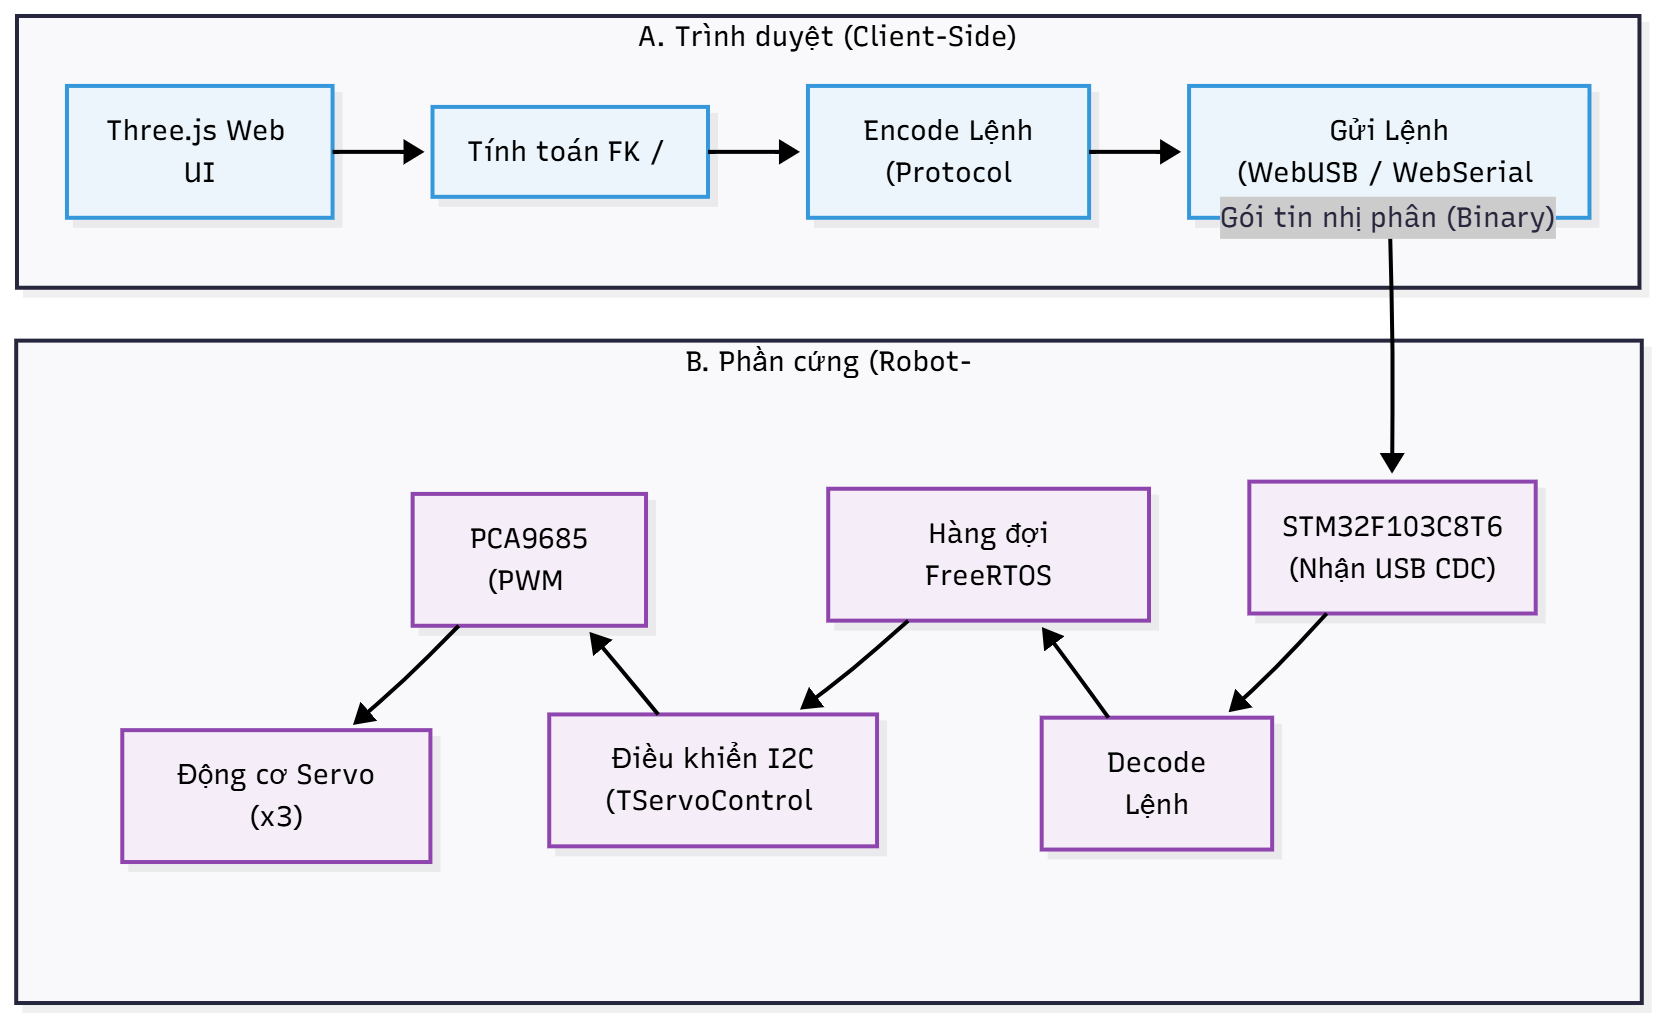
\includegraphics[height=\textwidth]{system-architecture.png}}
    \caption{Sơ đồ kiến trúc hệ thống tổng quan}
    \label{fig:system-architecture}
\end{figure}

Như thể hiện trong Hình \ref{fig:system-architecture}, các tác vụ tính toán nặng (FK/IK) được thực hiện ở phía trình duyệt. Vi điều khiển STM32 chỉ đóng vai trò nhận lệnh đã được mã hoá, giải mã và thực thi điều khiển PWM thông qua I2C.

%----- Luồng điều khiển -------------------------------------------------------
\section{Luồng điều khiển}

Luồng điều khiển (sequence flow) của một lệnh từ người dùng đến khi robot phản hồi được thể hiện trong Hình \ref{fig:sequence-diagram}.

\begin{figure}[H]
    \centering
    % Placeholder cho sơ đồ Mermaid
    {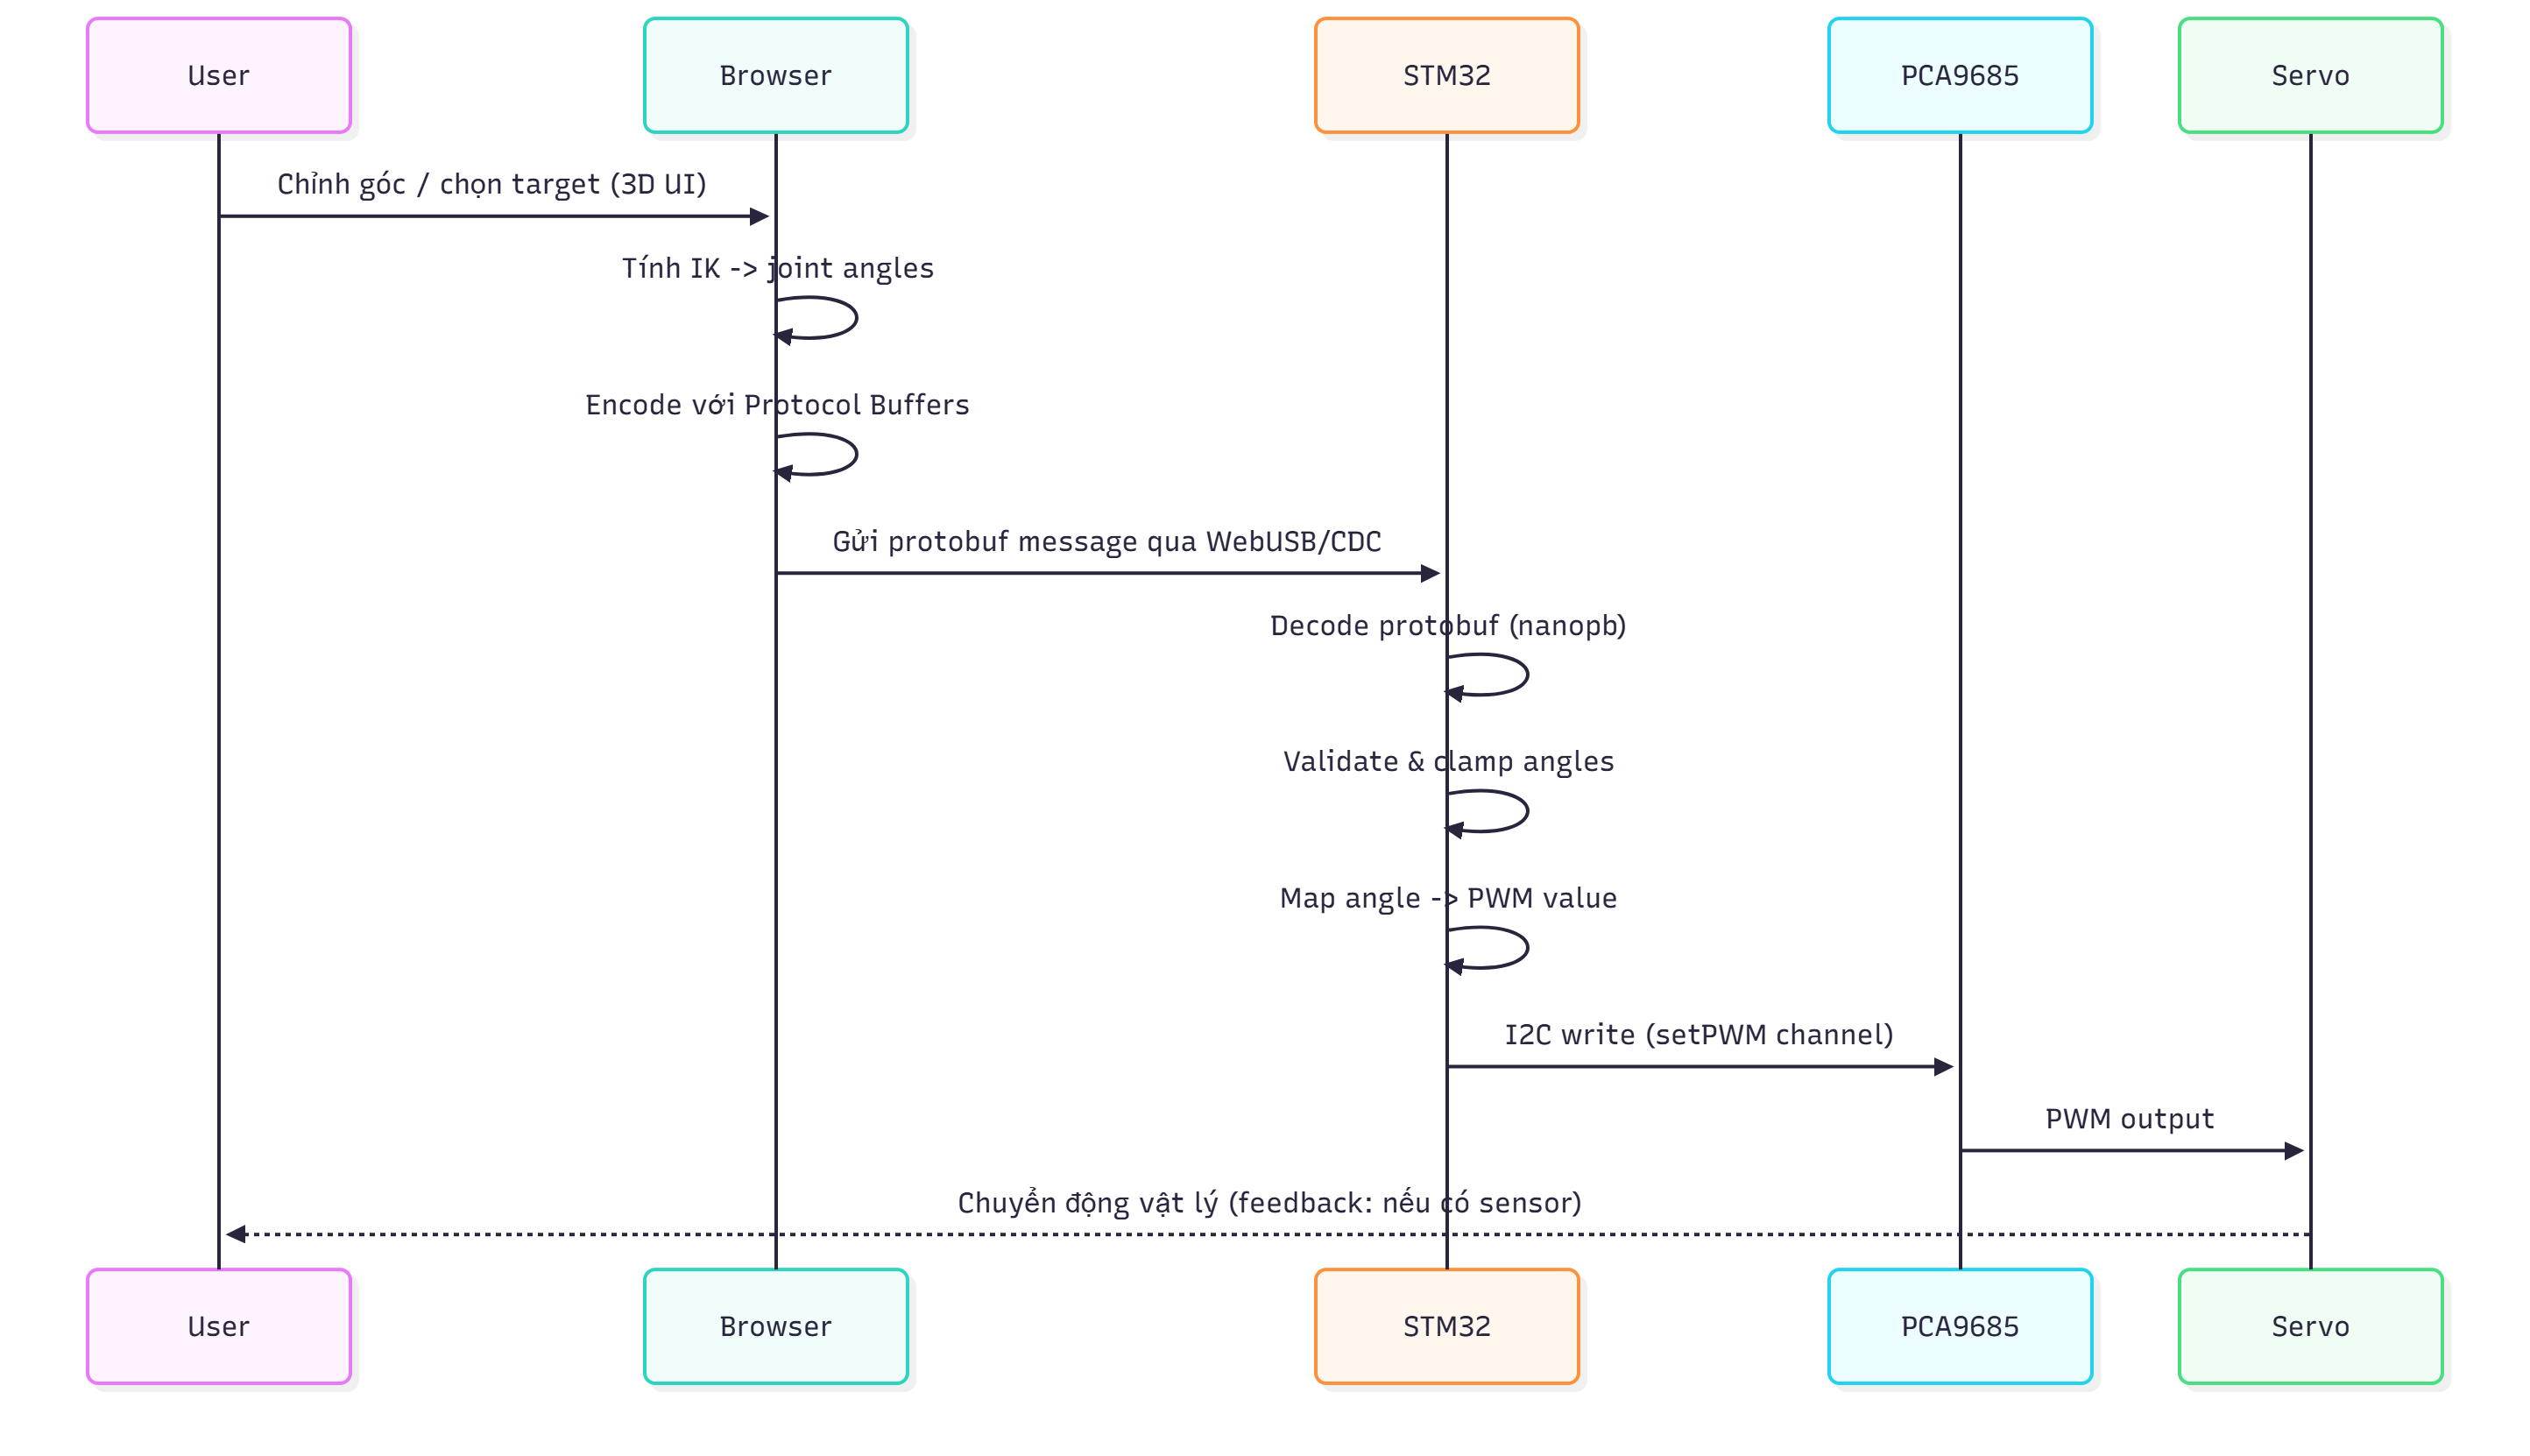
\includegraphics[width=\textwidth]{sequence-diagram.png}}
    \caption{Luồng điều khiển tuần tự (Sequence Diagram)}
    \label{fig:sequence-diagram}
\end{figure}

%----- Protocol Buffers -----------------------------------------------------
\section{Giao thức truyền thông: Protocol Buffers}

Để đảm bảo việc truyền dữ liệu giữa trình duyệt (TypeScript) và vi điều khiển (C) được đồng nhất, hiệu quả và an toàn, dự án sử dụng Protocol Buffers (Protobuf). Đây là một phương pháp tuần tự hoá (serialize) dữ liệu có cấu trúc do Google phát triển.

\subsection{Định nghĩa Message}
Cấu trúc gói tin được định nghĩa trong tệp `.proto`. Một gói tin `Message` chung sẽ bao bọc các loại payload cụ thể, ví dụ như `SetJointAngles`.

\begin{lstlisting}[language=protobuf, caption={Định nghĩa gói tin trong tệp \texttt{messages.proto}}, label={lst:proto-def}, float=H]
syntax = "proto3";
package openarm.v1;

message Message { // transport-agnostic envelope
  uint32 seq = 1;         // monotonic sequence
  uint64 timestamp_ms = 2; // unix ms (optional)
  
  oneof payload { // extensible
    Heartbeat heartbeat = 10;
    SetJointAngles set_joint_angles = 11;
    Ack ack = 12;
  }
}

message Heartbeat {}

enum Status {
  STATUS_OK = 0;
  STATUS_INVALID = 1;
  STATUS_OUT_OF_RANGE = 2;
  STATUS_TIMEOUT = 3;
  STATUS_I2C_ERROR = 4;
  STATUS_EMERGENCY_STOP = 5;
}

message Ack {
  uint32 seq_ack = 1;
  Status status = 2;
  string message = 3;
}

message SetJointAngles {
  float base_rad = 1;
  float shoulder_rad = 2;
  float elbow_rad = 3;
}
\end{lstlisting}


\subsection{Triển khai}
\begin{itemize}
    \item \textbf{Phía Web (Client):} Sử dụng `protoc-gen-es` (từ Buf) để biên dịch tệp `.proto` thành mã TypeScript (ES Module). Giao diện web sử dụng thư viện `@bufbuild/protobuf` để tạo và mã hoá (encode) các đối tượng message này thành một mảng `Uint8Array` nhị phân trước khi gửi qua WebUSB.
    \item \textbf{Phía Firmware (Device):} Sử dụng thư viện \textbf{nanopb}, một thư viện Protobuf siêu nhẹ dành cho C, để giải mã (decode) dữ liệu nhị phân nhận được từ USB CDC thành cấu trúc C (struct).
\end{itemize}

Việc này loại bỏ hoàn toàn nhu cầu phân tích (parse) chuỗi thủ công, giảm thiểu lỗi và tăng hiệu suất đáng kể.


%==============================================================================
% CHƯƠNG 3: THIẾT KẾ VÀ TRIỂN KHAI
%==============================================================================
\chapter{Thiết kế và Triển khai}

Chương này trình bày chi tiết về quá trình thiết kế cơ khí, lựa chọn linh kiện phần cứng, và kiến trúc phần mềm firmware chạy trên vi điều khiển STM32.

%----- Thiết kế cơ khí --------------------------------------------------------
\section{Thiết kế cơ khí}
Phần cơ khí của cánh tay robot 3DOF được thiết kế với mục tiêu tối ưu hoá hiệu năng của actuator và vật liệu gia công.

\subsection{Lựa chọn Actuator (Servo)}
Hệ thống sử dụng 3 động cơ servo MG90. Đây là lựa chọn cân bằng giữa chi phí và hiệu năng. Thông số kỹ thuật quan trọng nhất là mô-men xoắn:
\begin{itemize}
    \item \textbf{Mô-men xoắn (tải):} 1.8 kg/cm (tại 4.8V)
    \item \textbf{Góc quay:} 180 độ
\end{itemize}
Mô-men xoắn 1.8 kg/cm ($\sim$0.18 Nm) tại ngưỡng an toàn 4.8V được sử dụng làm thông số tiêu chuẩn để tính toán thiết kế.

\subsection{Tính toán thiết kế}
\subsubsection{Vật liệu}
Vật liệu được chọn là nhựa PETG, gia công bằng phương pháp in 3D. Lý do: Rẻ, nhẹ, và có cơ tính đủ tốt cho mô hình prototype.

\subsubsection{Tính toán chiều dài cánh tay}
Bài toán đặt ra là xác định chiều dài cánh tay ($r$) tối đa mà servo có thể nâng được, dựa trên trọng lượng cánh tay ($F$) và mô-men xoắn của servo ($M$).
Công thức cơ bản:
\begin{equation}
    \centering
    r_{\text{max}} = \frac{M}{F_{\text{min}}}
\end{equation}
Trong đó:
\begin{itemize}
    \item $M = 0.18$ Nm (Mô-men xoắn của servo MG90)
    \item $F_{\text{min}} \sim 0.1$ N (Trọng lượng ước tính của toàn bộ cánh tay, làm tròn lên để đảm bảo an toàn)
\end{itemize}

Thay số, ta có:
\begin{equation}
    \centering
    r_{\text{max}} = \frac{0.18 \text{ Nm}}{0.1 \text{ N}} = 1.8 \text{ m}
\end{equation}

Kết quả 1.8 m cho thấy servo có khả năng nâng cánh tay với chiều dài rất lớn. Tuy nhiên, để đảm bảo độ chính xác và độ cứng vững, thiết kế chọn tổng chiều dài 2 khớp là \textbf{20cm} (0.2m), mỗi khớp dài 10cm (0.1m).

\subsubsection{Khớp đế xoay 360 độ}
Servo MG90 chỉ có thể quay 180 độ. Để khớp đế (base) có thể xoay 360 độ, một hệ truyền động bánh răng với tỉ lệ 1:2 được sử dụng. Servo (gắn bánh răng lớn) truyền động cho phần đế (gắn bánh răng nhỏ). Khi servo quay 180 độ (1/2 vòng), đế sẽ quay 360 độ (1 vòng).

\subsection{Mô hình CAD}
Toàn bộ cơ cấu cánh tay robot được thiết kế trong phần mềm CAD (Onshape). Mô hình bao gồm các chi tiết chính: khớp đế (base), khớp vai (shoulder), khớp khuỷu (elbow), và các giá đỡ servo.

\begin{figure}[H]
    \centering
    {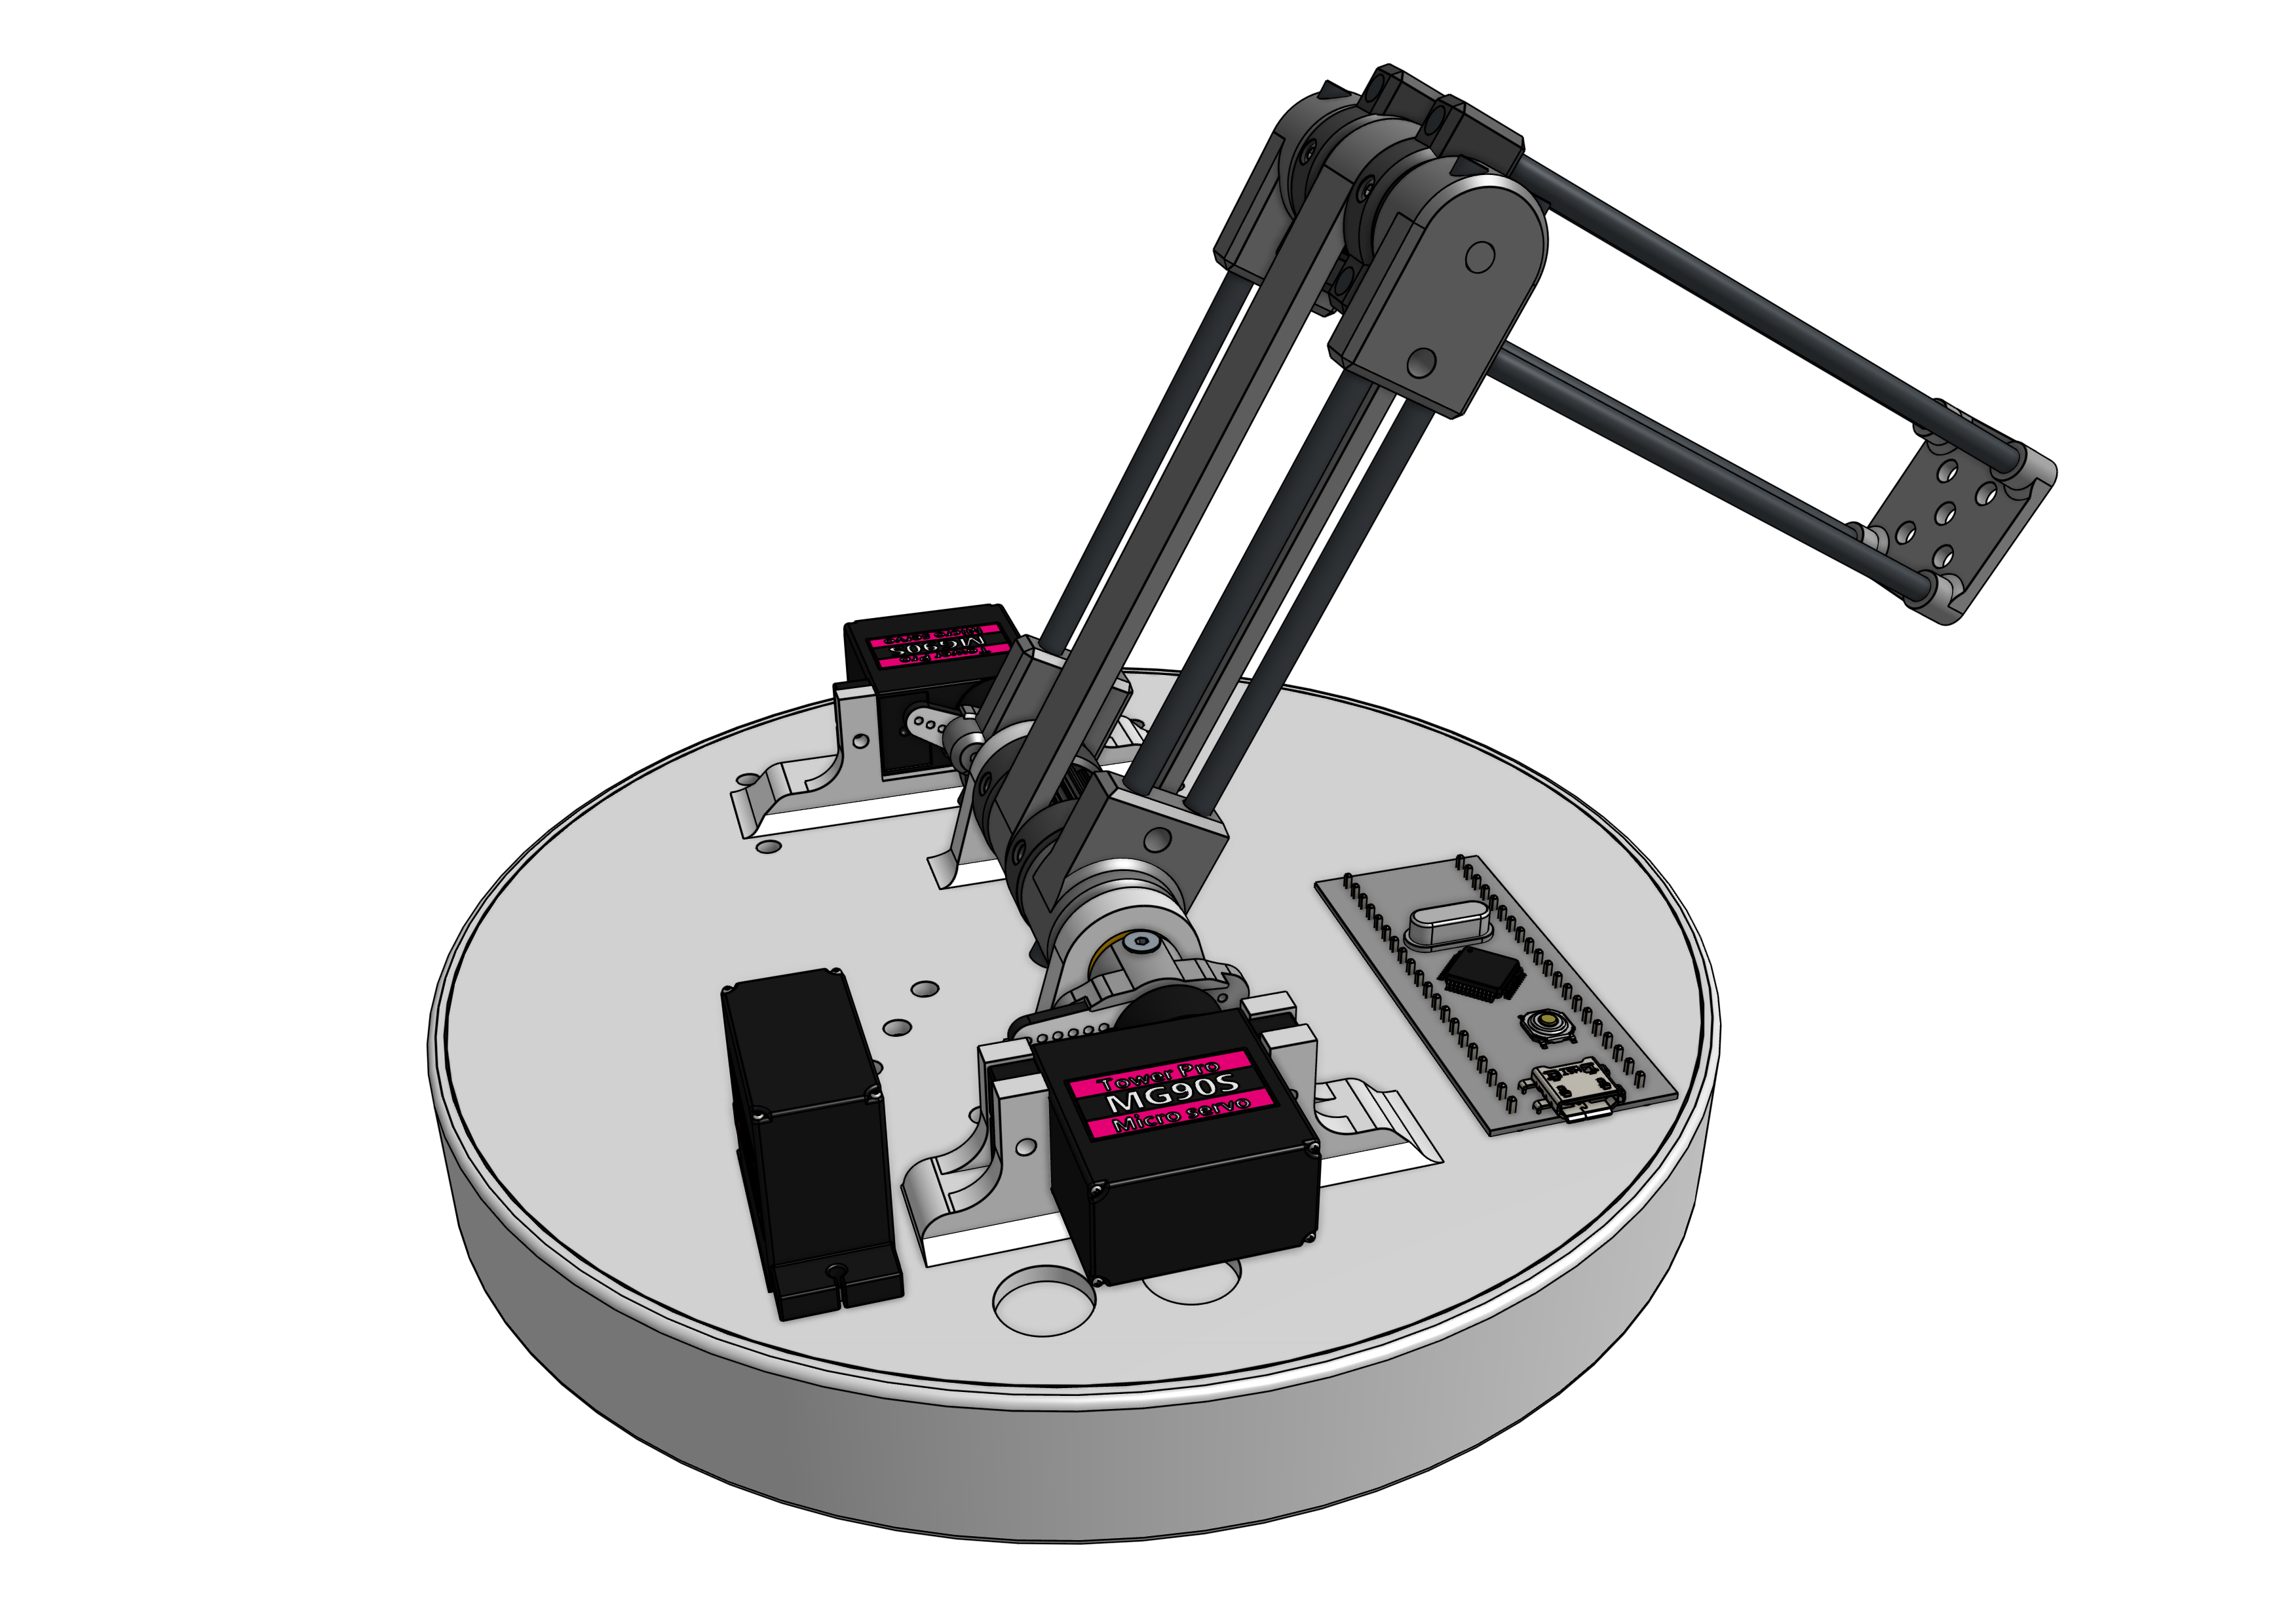
\includegraphics[width=0.8\textwidth]{mechanical-design-cad.png}}
    \caption{Mô hình CAD của cánh tay robot 3DOF}
    \label{fig:mechanical-cad}
\end{figure}

Hình \ref{fig:mechanical-cad} thể hiện mô hình CAD hoàn chỉnh của cánh tay robot, bao gồm cả hệ thống truyền động bánh răng cho khớp đế. Các chi tiết cánh tay robot sau đó được gia công bằng phương pháp in 3D nên được thiết kế để tối ưu hoá cho phương pháp này, với độ dày thành tối thiểu 2mm để đảm bảo độ bền.

%----- Thiết kế phần cứng -----------------------------------------------------
\section{Thiết kế phần cứng (Hardware)}

\subsection{Lựa chọn linh kiện}
\begin{itemize}
    \item \textbf{Vi điều khiển (MCU):} \textbf{STM32F103C8T6} (Blue Pill) được chọn vì có sẵn bộ xử lý USB (USB OTG) và hiệu năng đủ mạnh để chạy FreeRTOS và giải mã nanopb.
    \item \textbf{Driver Servo:} \textbf{PCA9685} được sử dụng thay vì dùng PWM trực tiếp từ STM32. Lý do: PCA9685 giao tiếp qua I2C, chỉ tốn 2 chân (SCL/SDA) của STM32 nhưng có thể điều khiển độc lập 16 kênh servo. Điều này giúp tiết kiệm tài nguyên MCU và rất dễ dàng cho việc mở rộng hệ thống sau này.
\end{itemize}

\subsection{Sơ đồ kết nối}
Hệ thống được kết nối theo sơ đồ trong Hình \ref{fig:hardware-wiring}.

\begin{figure}[H]
    \centering
    % Placeholder cho sơ đồ nối dây
    {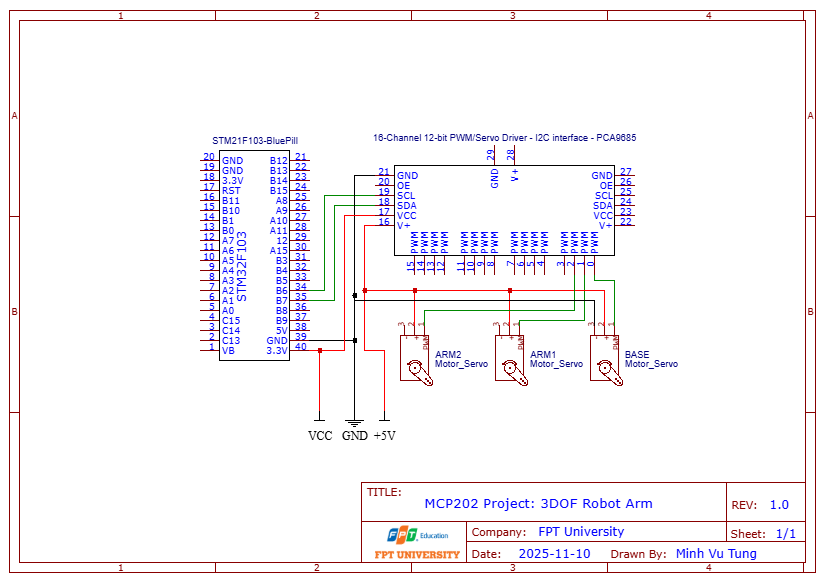
\includegraphics[width=\textwidth]{hardware-wiring.png}}
    \caption{Sơ đồ kết nối phần cứng (Minh họa)}
    \label{fig:hardware-wiring}
\end{figure}

%----- Thiết kế Firmware ----------------------------------------------------
\section{Thiết kế Firmware}

Firmware được xây dựng trên nền tảng STM32CubeMX và Keil MDK, sử dụng hệ điều hành thời gian thực FreeRTOS để quản lý các tác vụ.

\subsection{Kiến trúc FreeRTOS}
Hệ thống sử dụng 3 tác vụ (Task) chính chạy song song:

\begin{enumerate}
    \item \textbf{TProtocolParser (Normal Priority):}
    Chờ tín hiệu (Semaphore) từ ngắt USB. Khi có dữ liệu, Task này "thức dậy", lấy dữ liệu từ bộ đệm vòng (circular buffer), và gọi hàm \texttt{USB\_ProcessReceivedData}. Hàm này thực hiện giải mã (decode) gói tin Protobuf bằng nanopb.
    
    \item \textbf{TServoControl (High Priority):}
    Sau khi TProtocolParser giải mã thành công, nó đẩy lệnh (đã được validate) vào một hàng đợi (Message Queue) tên là \texttt{CommandQueueHandle}. Task TServoControl (ưu tiên cao) túc trực ở hàng đợi này. Ngay khi nhận được lệnh, nó gửi tín hiệu I2C đến PCA9685 để điều khiển servo.
    
    \item \textbf{TSafetyMonitor (Realtime Priority):}
    Task này giám sát thời gian nhận được lệnh cuối cùng. Nếu quá một khoảng thời gian (ví dụ: 2 giây) mà không có lệnh mới, nó sẽ tự động kích hoạt chế độ an toàn (ví dụ: ngắt PWM) để đảm bảo robot không gây nguy hiểm.
\end{enumerate}

\subsection{Mô hình xử lý ngắt ISR-to-Task}
Một cải tiến quan trọng trong firmware là cách xử lý dữ liệu từ USB.

\begin{itemize}
    \item \textbf{Phương pháp thông thường (Không khuyến khích):} Giải mã gói tin Protobuf ngay trong trình phục vụ ngắt USB (\texttt{CDC\_Receive\_FS}). Điều này rất nguy hiểm vì ISR cần chạy cực kỳ nhanh. Nếu gói tin lỗi hoặc việc giải mã tốn thời gian, nó có thể làm "treo" toàn bộ hệ thống.
    
    \item \textbf{Phương pháp cải tiến (ISR-to-Task):}
    Khi ngắt USB (\texttt{CDC\_Receive\_FS}) được kích hoạt, nó chỉ thực hiện hai việc siêu nhanh:
    \begin{enumerate}
        \item Copy dữ liệu mới nhận vào một bộ đệm vòng (circular buffer).
        \item "Báo hiệu" (release) một \textbf{Semaphore} (\texttt{UsbDataAvailableHandle}).
    \end{enumerate}
    Task \texttt{TProtocolParser} (là một Task bình thường, không phải ISR) sẽ "chờ" (acquire) Sempahore này. Khi được báo hiệu, nó mới bắt đầu quá trình giải mã gói tin. Phương pháp này đảm bảo ISR không bao giờ bị nghẽn và hệ thống ổn định hơn rất nhiều.
\end{itemize}


%==============================================================================
% CHƯƠNG 4: KẾT QUẢ VÀ HẠN CHẾ
%==============================================================================
\chapter{Kết quả và Hạn chế}

%----- Giao diện Web ---------------------------------------------------------
\section{Giao diện Web (Webconnect)}

Giao diện người dùng (UI) được xây dựng trên nền tảng SvelteKit và Three.js, cung cấp một phương pháp trực quan hoá và tối ưu trải nghiệm người dùng.

Các tính năng chính của giao diện web:
\begin{itemize}
    \item \textbf{Hiển thị 3D:} Tích hợp mô hình 3D (định dạng URDF) của cánh tay robot, cho phép người dùng xoay, zoom và tương tác trực quan.
    \item \textbf{Kết nối phần cứng:} Sử dụng Web Serial API để tự động phát hiện và kết nối với STM32 qua cổng USB CDC (Virtual COM Port).
    \item \textbf{Tải tài nguyên:} Toàn bộ tài nguyên (asset) 3D (tệp URDF, STL) được tải từ CDN (Cloudflare R2) thông qua một tệp `manifest.json`.
\end{itemize}

\begin{figure}[H]
    \centering
    % Placeholder cho ảnh giao diện
    {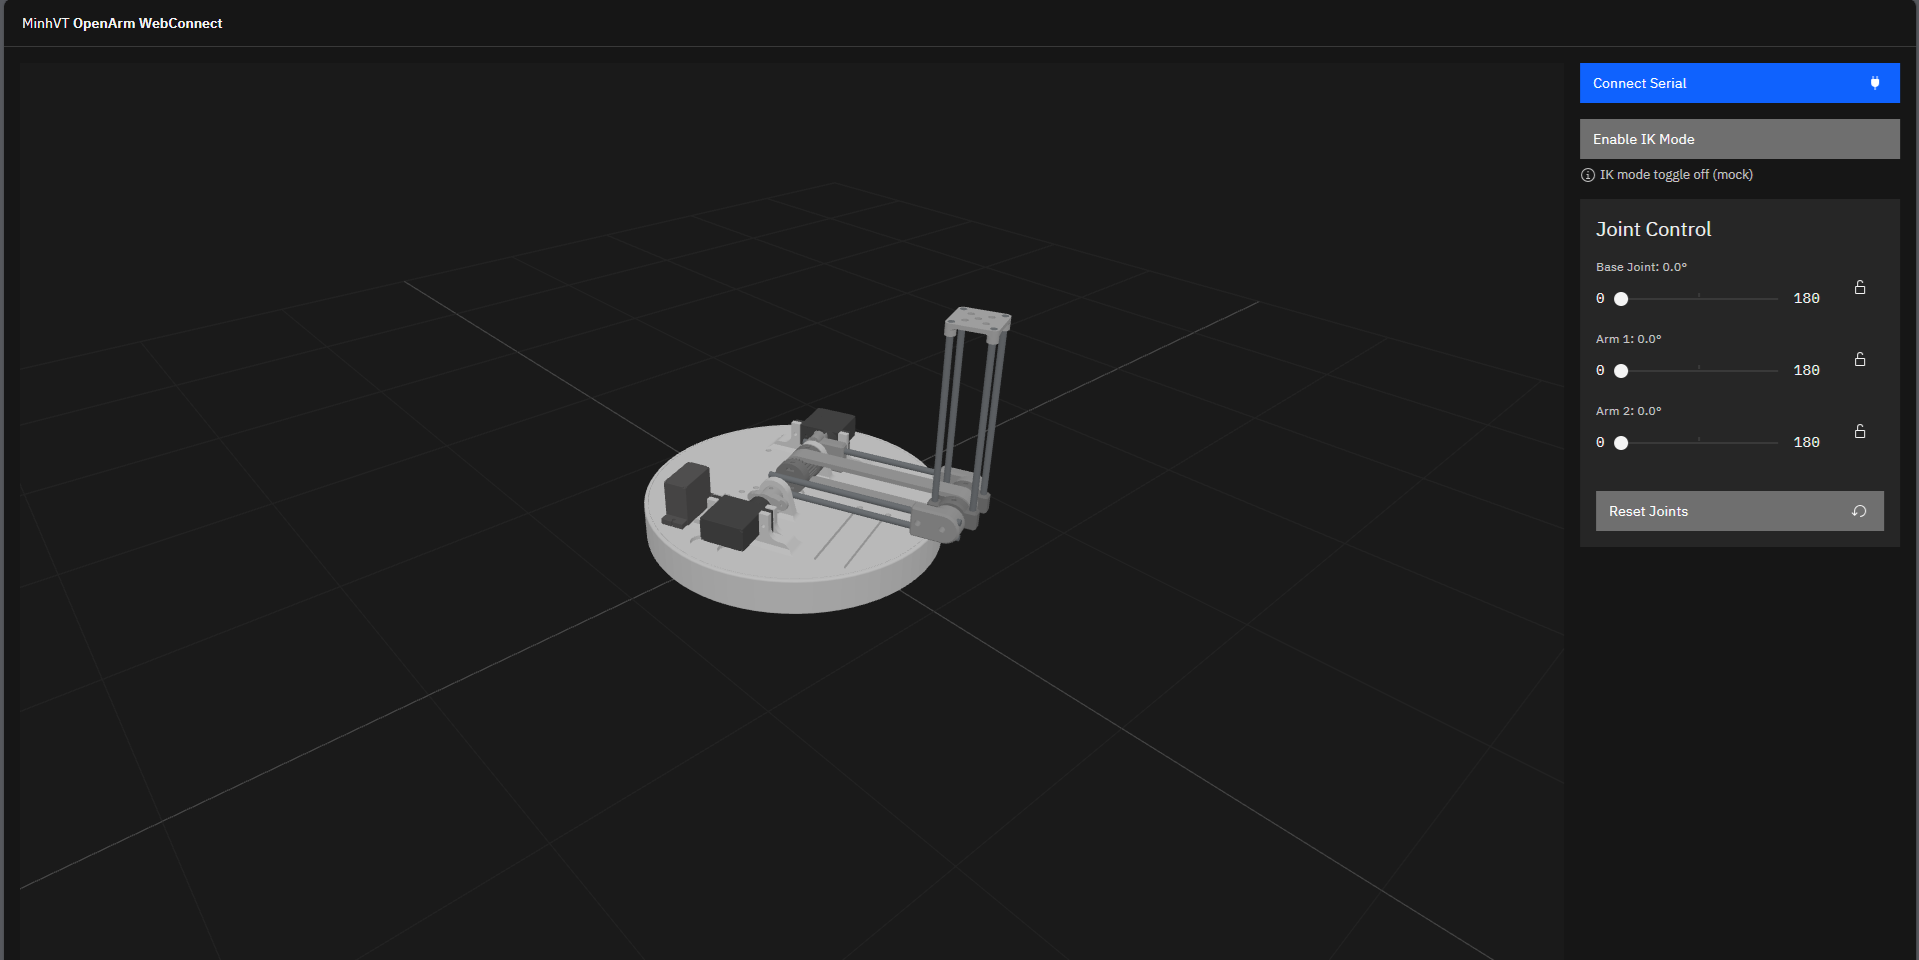
\includegraphics[width=\textwidth]{web-ui.png}}
    \caption{Giao diện điều khiển WebConnect (Minh họa)}
    \label{fig:web-ui}
\end{figure}

\section{Chế độ điều khiển}

Giao diện web hỗ trợ hai chế độ điều khiển chính:

\begin{enumerate}
    \item \textbf{Động học thuận (Forward Kinematics - FK):}
    Người dùng điều khiển trực tiếp từng góc quay của khớp (base, arm1, arm2) thông qua các thanh trượt (sliders). Giao diện sẽ gửi góc (đã chuyển đổi sang radian) đến vi điều khiển.
    
    \item \textbf{Động học nghịch (Inverse Kinematics - IK):}
    Người dùng "bật" chế độ IK. Khi đó, thanh trượt bị vô hiệu hoá. Một mục tiêu 3D (transform control) xuất hiện. Người dùng có thể kéo/thả mục tiêu này đến vị trí mong muốn trong không gian. 
    
    Toàn bộ phép toán IK (sử dụng giải thuật CCD) được thực thi ngay trên trình duyệt (phía client) để tính toán ra 3 góc khớp cần thiết. Các góc này sau đó được gửi đến vi điều khiển.
\end{enumerate}

Phương pháp "tính toán tại phía người dùng" này giúp giảm tải tối đa cho vi điều khiển, đảm bảo vi xử lý STM32 không bị quá tải và chỉ tập trung vào việc thực thi lệnh theo thời gian thực.

%----- Hạn chế ---------------------------------------------------------------
\section{Hạn chế của dự án}

Mặc dù hệ thống đã hoạt động, vẫn còn một số hạn chế:
\begin{itemize}
    \item \textbf{Điều khiển vòng hở (Open Loop):} Hệ thống hiện tại là vòng điều khiển hở. Vi điều khiển "ra lệnh" cho servo quay 90 độ và "tin" là nó sẽ quay 90 độ, chứ không có cảm biến phản hồi (như encoder hay biến trở) ở khớp để đo xem nó có thật sự quay đúng 90 độ hay không.
    \item \textbf{Giao tiếp một chiều:} Giao tiếp hiện tại chủ yếu là 1 chiều (Web $\rightarrow$ Robot). Firmware chưa triển khai việc gửi thông điệp phản hồi (ACK) ngược về trình duyệt để xác nhận "đã nhận được lệnh" hay "lệnh bị lỗi".
    \item \textbf{Hạn chế mô phỏng web:} Giao diện web 3D (Three.js) chưa mô phỏng chân thật các yếu tố vật lý như va chạm. Đây là một sự đánh đổi để tăng khả năng tiếp cận (cross-platform) và dễ dàng phát hành sản phẩm so với các engine native như PyBullet hay MuJoCo.
\end{itemize}

%==============================================================================
% CHƯƠNG 5: KẾT LUẬN VÀ HƯỚNG PHÁT TRIỂN
%==============================================================================
\chapter{Kết luận và Hướng phát triển}

%----- Kết luận --------------------------------------------------------------
\section{Kết luận}

Đồ án đã hoàn thành các mục tiêu chính đề ra, xây dựng thành công một hệ thống điều khiển cánh tay robot 3DOF hoàn chỉnh, bao gồm:
\begin{enumerate}
    \item \textbf{Thiết kế cơ khí:} Hoàn thiện mô hình cơ khí 3DOF, tối ưu hoá cho vật liệu in 3D và giải quyết được bài toán xoay 360 độ cho khớp đế.
    \item \textbf{Thiết kế phần cứng:} Lựa chọn và kết nối thành công vi điều khiển STM32F103C8T6 với driver PWM PCA9685 qua I2C.
    \item \textbf{Phát triển Firmware:} Xây dựng firmware trên nền tảng FreeRTOS, áp dụng mô hình ISR-to-Task để xử lý dữ liệu USB một cách ổn định. Tích hợp thành công thư viện nanopb để giải mã các gói tin Protocol Buffers.
    \item \textbf{Phát triển Giao diện Web:} Hoàn thiện ứng dụng WebConnect (SvelteKit + Three.js) có khả năng hiển thị URDF, tính toán IK/FK phía client và truyền lệnh điều khiển qua Web Serial API.
\end{enumerate}

Sự kết hợp giữa WebUSB, Protocol Buffers, và FreeRTOS đã chứng minh là một giải pháp hiệu quả, mạnh mẽ và có khả năng mở rộng để kết nối các ứng dụng web hiện đại với các hệ thống nhúng thời gian thực.

%----- Hướng phát triển -------------------------------------------------------
\section{Hướng phát triển}

Dựa trên các hạn chế đã nêu, các hướng phát triển và nâng cấp trong tương lai bao gồm:
\begin{itemize}
    \item \textbf{Điều khiển vòng kín (Closed Loop):} Nâng cấp thiết kế cơ khí bằng cách thêm cảm biến phản hồi (biến trở hoặc encoder) tại mỗi khớp để đo góc quay thực tế.
    \item \textbf{Giao tiếp hai chiều:} Hoàn thiện giao thức Protobuf, cho phép STM32 gửi các gói tin `Ack` (xác nhận) hoặc gói tin `Telemetry` (chứa dữ liệu cảm biến) ngược trở lại trình duyệt để hiển thị trạng thái robot theo thời gian thực.
    \item \textbf{An toàn (Safety):} Cải tiến `TSafetyMonitor` để xử lý các trạng thái lỗi phức tạp hơn và ngắt servo khi có sự cố timeout.
\end{itemize}

%==============================================================================
% PHỤ LỤC
%==============================================================================
\appendix % Bắt đầu phần phụ lục
\cleardoublepage
\renewcommand{\thefigure}{\Alph{chapter}.\arabic{figure}}
\renewcommand{\thetable}{\Alph{chapter}.\arabic{table}}
\renewcommand{\thelstlisting}{\Alph{chapter}.\arabic{lstlisting}}

%----- Phụ lục A --------------------------------------------------------------
\chapter{Mã nguồn tích hợp Giao diện Web}
\label{app:web-integration}

Phần phụ lục này trích dẫn các đoạn mã quan trọng, minh họa cách giao diện web (TypeScript) kết nối và gửi dữ liệu đến STM32.

\section{Kết nối thiết bị (WebSerial API)}
Hàm `connect()` sử dụng `navigator.serial.requestPort` để yêu cầu người dùng chọn cổng COM ảo (USB CDC) của STM32.

\begin{lstlisting}[language=TypeScript, caption={Hàm kết nối WebSerial API}, label={lst:web-connect}, float=H]
import { openarm } from '@openarm/proto-es';

export class RobotArm {
  private port: SerialPort | null = null;
  private writer: WritableStreamDefaultWriter<Uint8Array> | null = null;
  private reader: ReadableStreamDefaultReader<Uint8Array> | null = null;
  private sequence = 0;
  public isConnected = false;

  async connect() {
    try {
      this.port = await navigator.serial.requestPort({
        // Filter for STMicroelectronics devices
        filters: [{ usbVendorId: 0x0483, usbProductId: 0x5740 }],
      });
      await this.port.open({ baudRate: 115200 });
      
      this.writer = this.port.writable!.getWriter();
      this.reader = this.port.readable!.getReader();
      this.isConnected = true;
      
      console.log('Connected to Open Arm');
      // this.startReadLoop(); // Will open when having ACK
    } catch (err) {
      console.error('Connection failed:', err);
    }
  }
  
  // ... (disconnect and other methods) ...
}
\end{lstlisting}

\section{Mã hoá và Gửi lệnh}
Hàm `setJoints()` tạo một đối tượng message `SetJointAngles`, mã hoá nó bằng `.toBinary()` (từ thư viện Protobuf-ES) và gửi mảng byte qua `writer.write()`.

\begin{lstlisting}[language=TypeScript, caption={Hàm mã hoá và gửi lệnh SetJointAngles}, label={lst:web-send}, float=H]
  async setJoints(baseRad: number, shoulderRad: number, elbowRad: number) {
    if (!this.writer) {
      throw new Error('Not connected');
    }

    // 1. Create message object
    const message = new openarm.v1.Message({
      seq: this.sequence++,
      timestampMs: BigInt(Date.now()),
      payload: {
        case: 'setJointAngles',
        value: new openarm.v1.SetJointAngles({
          baseRad,
          shoulderRad,
          elbowRad,
        }),
      },
    });

    // 2. Encode to Uint8Array
    const buffer = message.toBinary();
    
    // 3. Send via WebSerial
    await this.writer.write(buffer);
  }
\end{lstlisting}

%==============================================================================
% TÀI LIỆU THAM KHẢO
%==============================================================================
\cleardoublepage
\addcontentsline{toc}{chapter}{Tài liệu tham khảo}
\markboth{TÀI LIỆU THAM KHẢO}{}
\begin{thebibliography}{9}
\label{sec:references}

% [1] Nguồn mã nguồn dự án
\bibitem{openarm_repo}
Minh Vu Tung, "OpenArm: A 3-DOF robot arm control system," 2025. [Online]. Available: \url{https://github.com/thuongton999/openarm}

% [2] Tham khảo từ tệp dự án (Nanopb)
\bibitem{nanopb_docs}
P. Aimonen, "Nanopb - Protocol Buffers for Embedded Systems," [Online]. Available: \url{https://jpa.kapsi.fi/nanopb/}

% [3] Tham khảo từ tệp dự án (Web Serial API)
\bibitem{mdn_webserial_2024}
MDN Web Docs, "Web Serial API," Mozilla Developer Network, 2024. [Online]. Available: \url{https://developer.mozilla.org/en-US/docs/Web/API/Web_Serial_API}

% [4] Tham khảo từ tệp dự án (STM32)
\bibitem{stm32_docs}
STMicroelectronics, "STM32F103C8T6 Datasheet," [Online]. Available: \url{https://www.st.com/resource/en/datasheet/stm32f103c8.pdf}

\end{thebibliography}

\end{document}